\documentclass[11pt,letterpaper]{article}
\usepackage[T1]{fontenc}
\usepackage{lmodern}
\usepackage[utf8]{inputenc}
\usepackage[margin=2.35cm]{geometry}
\usepackage{booktabs,graphicx,hyperref}
\hypersetup{hidelinks}
\setlength{\parindent}{0pt}
\setlength{\parskip}{0.55em}
\renewcommand{\figurename}{Figura}
\begin{document}
{\small Instituto Politécnico Nacional $\cdot$ Escuela Superior de Cómputo\\Procesamiento de Lenguaje Natural $\cdot$ Noviembre de 2026}
\section*{Clasificación de sentimiento en reseñas de Steam}
\textbf{Proyecto de recuperación de opiniones, etapa II}\\
García Valiente Ángel René, Cabello Cárdenas Ulises Abdiel y Mexica Contreras Yaretzi

\textbf{Resumen.} ¿Permiten las palabras de una reseña predecir si su autor recomienda el juego? Se compararon 132 configuraciones sobre 600 reseñas de Steam. En desarrollo, la regresión logística y el clasificador de margen lineal alcanzaron el mismo macro-F1 (0.8113). La configuración seleccionada combinó frecuencias de palabras con cuatro rasgos de polaridad. En prueba acertó 80 de 90 votos y recuperó seis de las catorce recomendaciones negativas.
\section{Corpus, etiquetas y particiones}
Se reutilizó el corpus congelado de la etapa I, con 100 reseñas en inglés por cada uno de seis videojuegos. La unidad de análisis es la reseña. Su identificador se conserva como \texttt{document\_id} y su texto original como \texttt{text}. Steam registra una recomendación binaria en \texttt{voted\_up}. El valor verdadero se tradujo a \textit{positive} y el falso a \textit{negative}. El corpus contiene 600 textos e identificadores distintos. La auditoría registró cero calificaciones vacías, etiquetas fuera de los dos valores admitidos y reseñas vacías. El predictor recibe exclusivamente el texto. La calificación y el juego quedan como metadatos.

\begin{center}\begin{tabular}{lrrrr}\toprule
Partición & Negativas & Positivas & Total & Negativas (\%)\\\midrule
Entrenamiento &64&356&420&15.24\\
Desarrollo &13&77&90&14.44\\
Prueba &14&76&90&15.56\\\midrule
Corpus &91&509&600&15.17\\\bottomrule\end{tabular}\end{center}

Se barajaron las reseñas con semilla 0 y se estratificó por etiqueta para mantener representada la clase minoritaria en las tres particiones. El vocabulario, los pesos y las transformaciones que requieren ajuste se estimaron con entrenamiento durante la selección. Se reservó desarrollo para comparar opciones. Tras congelar C080 se reajustó con las 510 reseñas de entrenamiento y desarrollo y se evaluó la configuración final una vez en prueba.

La recomendación resume una decisión del usuario que puede diferir del tono de una frase. Por ejemplo, la reseña 238204926 combina «I hate this game» con la admisión de que juega a diario. La revisión manual documentó la ambigüedad y conservó el voto positivo original. Cambiarlo por intuición habría modificado la tarea supervisada.


\newpage
\section{Cómo se construye el pipeline}
La función \texttt{construir\_pipeline} de \texttt{preprocesamiento.py} recibe una configuración experimental. En la rama de texto, \texttt{Normalizador} entrega tokens separados por espacios y el vectorizador conserva los tokens tal como los recibe. Según el ensayo se emplean conteos, presencia binaria o TF--IDF con unigramas, bigramas o ambos. En una rama paralela, cada recurso lingüístico recibe la reseña y devuelve dos valores. \texttt{FeatureUnion} concatena las columnas y \texttt{ClasificadorBalanceado} ajusta el estimador con la estrategia de entrenamiento indicada.

Por ejemplo, en C080 las contracciones hacen explícita la negación. La rama de unigramas conserva el negador y cuenta palabras. Por separado, en una expresión como \textit{not good}, las ramas léxicas intercambian los puntajes positivo y negativo de la palabra bajo negación. Así se distingue conservar el token \textit{not} de marcarlo en el vocabulario y de invertir la polaridad en los rasgos adicionales.

\subsection*{De la línea base a la selección}
\begin{enumerate}
\item \textbf{E1.} Con frecuencias de unigramas se parte de tokenización sola. Se ensayan individualmente limpieza, contracciones, repeticiones, ortografía, lematización y eliminación de palabras vacías. Para regresión logística, explicitar contracciones elevó el macro-F1 de 0.6427 (C038) a 0.7750 (C040).
\item \textbf{E2.} Se combinan los pasos prometedores y se prueban combinaciones explícitas de ortografía y repeticiones. Con regresión logística, repeticiones más ortografía (C056) obtuvo 0.6427, igual que la tokenización sola y por debajo de C040. En la auditoría ortográfica, la primera versión transformaba el nombre \textit{Wingull} en \textit{lingual}. Al proteger vocabulario, el macro-F1 de LinearSVC con ortografía sola pasó de 0.7574 a 0.7035. Una sustitución que favorece la puntuación puede deteriorar el significado de la reseña.
\item \textbf{E3 y E4.} Se comparan estrategias de desbalance y después representaciones. TruncatedSVD se ensaya con 100 y 300 componentes en regresión logística y LinearSVC. La proyección puede producir coordenadas negativas, incompatibles con el modelo multinomial. La configuración ganadora conserva las frecuencias de unigramas en su espacio original.
\item \textbf{E5 y E6.} Se fija una referencia sin aumento lingüístico para cada familia. Se ensayan los recursos por separado y se combinan los dos mejor situados. El cuadro de la página siguiente permite distinguir los aportes individuales de las interacciones.
\item \textbf{E7.} \texttt{Registro.rejilla} ejecuta \texttt{GridSearchCV} con \texttt{PredefinedSplit}: entrenamiento para estimar parámetros y desarrollo para puntuar. Se prueban $\alpha\in\{0.01,0.1,0.5,1,2\}$ en Naive Bayes y $C\in\{0.01,0.1,1,10,100\}$ en los clasificadores lineales. Se trata de una búsqueda por etapas: el resultado depende también de qué variantes sobrevivieron a cada comparación.
\end{enumerate}
\newpage
\section{Qué aportaron los recursos lingüísticos}
Las listas de Hu y Liu cuentan palabras positivas y negativas. El recurso compacto de SentiWordNet 3.0 promedia las polaridades de los sentidos de cada palabra con pesos inversos a su número de sentido y omite expresiones de varias palabras. En ambos casos, la negación local intercambia las dos polaridades. Cada suma se transforma con $\log(1+x)$ para moderar el peso de reseñas largas. El catálogo de emojis del curso y las listas de emoticonos proporcionan otra pareja de rasgos. Su cobertura en entrenamiento fue de 3.8\%, frente a 88.6\% de Hu y Liu y 99.0\% de SentiWordNet. Reconocer una palabra tampoco garantiza interpretar su sentido en videojuegos.
\begin{center}\small\begin{tabular}{lrrr}\toprule
Macro-F1 en desarrollo & NB & Reg. logística & LinearSVC\\\midrule
Referencia sin aumento & 0.6684 & 0.7750 & 0.7910\\
Marcar negación & 0.7340 & 0.7574 & 0.7929\\
Eliminar negadores & 0.6181 & 0.6427 & 0.7188\\
Hu y Liu & 0.6296 & 0.7929 & 0.7910\\
SentiWordNet & 0.6023 & 0.7750 & 0.8113\\
Emojis y emoticonos & 0.6584 & 0.7750 & 0.7910\\
Dos mejores de cada familia & 0.7222 & 0.8113 & 0.7929\\\bottomrule\end{tabular}\end{center}
En regresión logística, combinar Hu y Liu con SentiWordNet añadió 0.0363 al macro-F1 y 0.0667 al F1 negativo frente a C040. SentiWordNet solo había empatado con la referencia. En Naive Bayes, combinar negación y emojis rindió menos que marcar solo la negación. En LinearSVC, SentiWordNet solo superó a la combinación con negación. Eliminar negadores perjudicó a las tres familias.

\subsection*{Desbalance y fuga de información}
La minoría representa 91 de las 600 reseñas. Se diagnosticó antes de dividir los datos. Durante los ensayos, el remuestreo se aplicó únicamente al ajustar el clasificador con entrenamiento. En regresión logística, el macro-F1 de 0.7750 pasó a 0.7596 con ponderación, 0.7574 con sobremuestreo aleatorio, 0.5537 con submuestreo y 0.5570 con SMOTE. Este último interpola vectores vecinos: la combinación de coordenadas dispersas carece de garantía de corresponder a una frase real. El modelo final conservó la distribución observada.

Una demostración independiente con entrenamiento y desarrollo ilustra el peligro de invertir el orden. Al sobremuestrear antes de dividir, 77 de 153 reseñas de evaluación se repitieron en entrenamiento y el macro-F1 aparente alcanzó 0.9673. Con partición previa hubo cero solapamientos. Los tamaños distintos impiden interpretar la diferencia como ganancia de un método.
\newpage
\section{Elección del modelo y resultados finales}
En cada familia se conserva el primer ensayo que alcanza el máximo macro-F1 redondeado a cuatro decimales. Entre ganadores se compara primero macro-F1 y luego F1 negativo. C080 y C125 empataron también en F1 negativo (0.6667). La función \texttt{max} conservó la regresión logística por el orden de recorrido. La selección quedó registrada en \texttt{modelos/config\_final.json} antes del reajuste con 510 reseñas.
\begin{center}\small\begin{tabular}{llrrrr}\toprule
Conjunto & ID & Exactitud & Prec. macro & Recall macro & Macro-F1\\\midrule
dev & C035 & 0.8444 & 0.7164 & 0.8132 & 0.7462\\
dev & C080 & 0.9222 & 0.9009 & 0.7627 & 0.8113\\
dev & C125 & 0.9222 & 0.9009 & 0.7627 & 0.8113\\
test & test & 0.8889 & 0.8262 & 0.7011 & 0.7411\\\bottomrule\end{tabular}\end{center}
C035 (Naive Bayes) usó todos los pasos de normalización, TF--IDF con unigramas y bigramas, negación marcada, ponderación y $\alpha=0.5$. C125 (LinearSVC) usó contracciones, filtrado de palabras vacías, unigramas de frecuencia y SentiWordNet. C080 usó contracciones, unigramas de frecuencia, Hu y Liu y SentiWordNet. Los dos clasificadores lineales conservaron $C=1$.
\begin{center}\small\begin{tabular}{llrrr|rrr}\toprule
ID & Partición & Prec. neg. & Recall neg. & F1 neg. & Prec. pos. & Recall pos. & F1 pos.\\\midrule
C035 & dev & 0.476 & 0.769 & 0.588 & 0.957 & 0.857 & 0.904\\
C080 & dev & 0.875 & 0.538 & 0.667 & 0.927 & 0.987 & 0.956\\
C125 & dev & 0.875 & 0.538 & 0.667 & 0.927 & 0.987 & 0.956\\
test & test & 0.750 & 0.429 & 0.545 & 0.902 & 0.974 & 0.937\\\bottomrule\end{tabular}\end{center}
En prueba, el clasificador recuperó 6 de 14 negativas y 74 de 76 positivas. Si se toma la recomendación negativa como la clase de interés, hubo ocho críticas omitidas y dos falsas alarmas. Predecir siempre la clase mayoritaria habría acertado 76 de 90. El macro-F1 cayó de 0.8113 a 0.7411 y el número reducido de negativas obliga a interpretar el recall con cautela.
\begin{center}
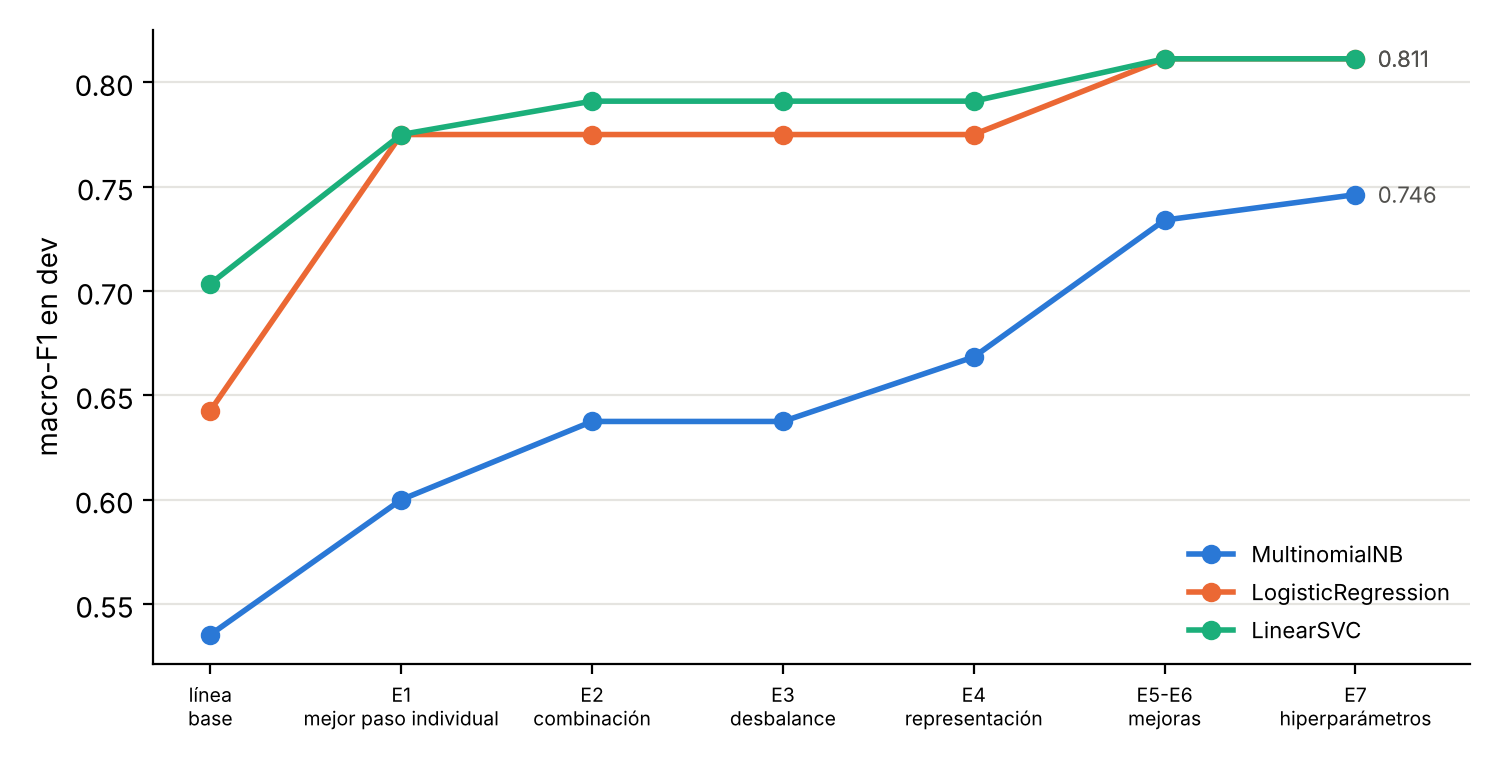
\includegraphics[width=.72\linewidth]{codigo_etapa2/resultados/figuras/progreso_por_etapa.png}\\
{\small Evolución de las configuraciones retenidas en desarrollo.}
\end{center}
\newpage
\section{Matrices de confusión y errores de desarrollo}
\begin{center}
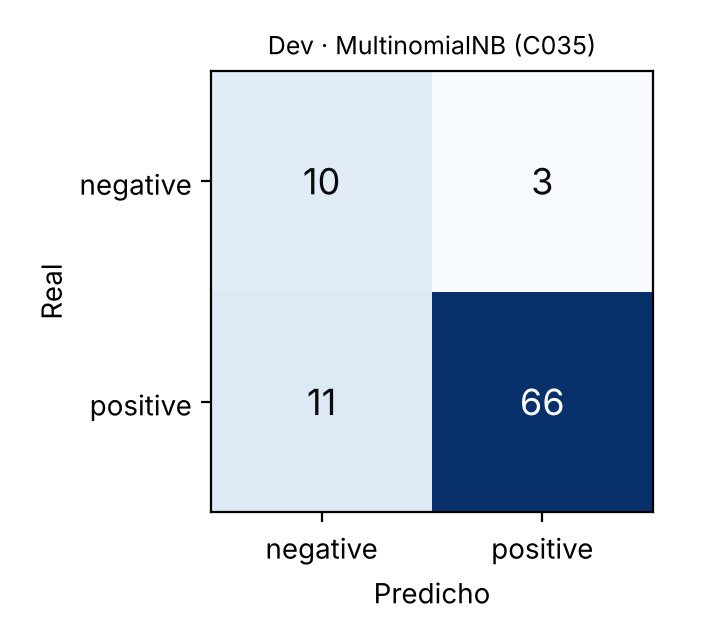
\includegraphics[width=.34\linewidth]{codigo_etapa2/resultados/figuras/matriz_dev_MultinomialNB.png}
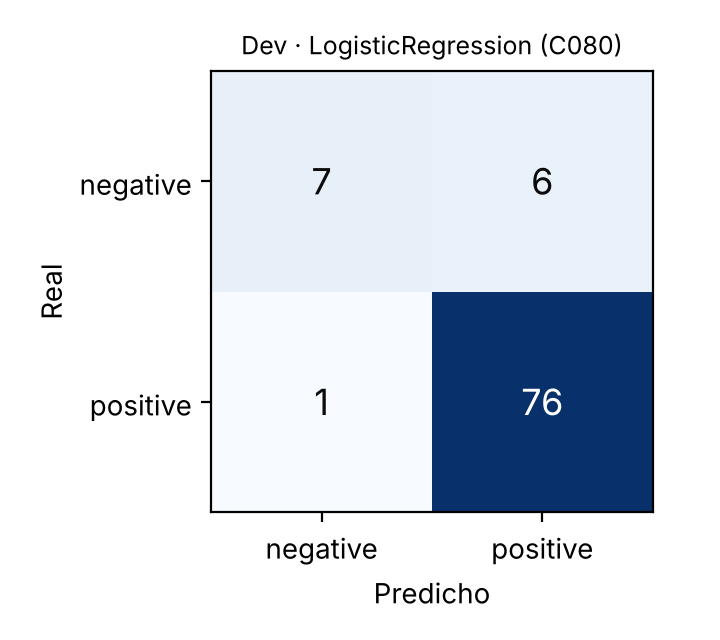
\includegraphics[width=.34\linewidth]{codigo_etapa2/resultados/figuras/matriz_dev_LogisticRegression.png}\\
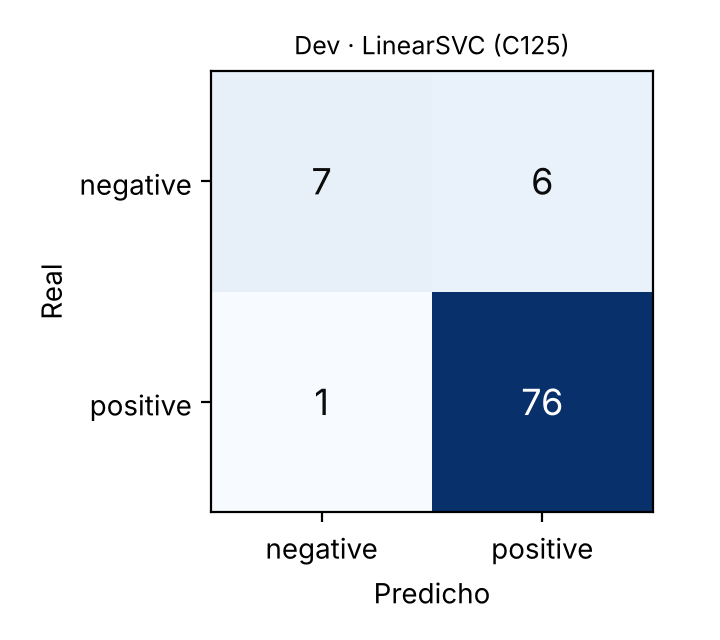
\includegraphics[width=.34\linewidth]{codigo_etapa2/resultados/figuras/matriz_dev_LinearSVC.png}
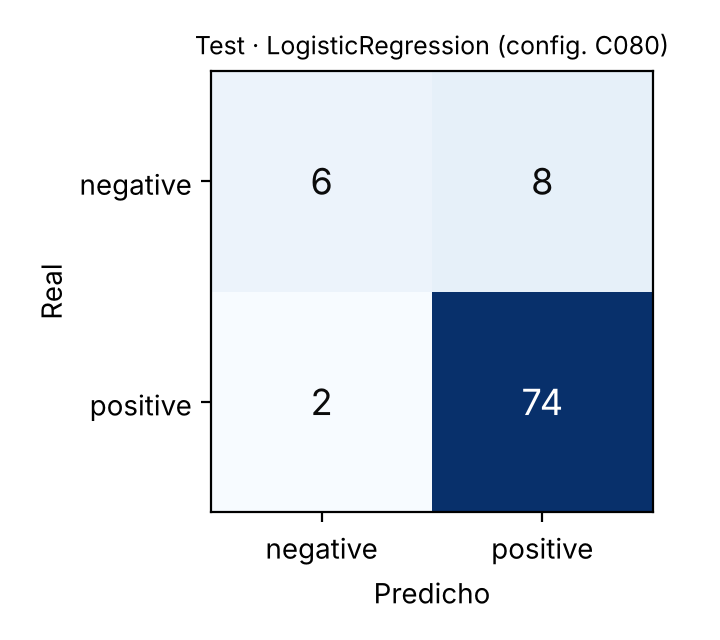
\includegraphics[width=.34\linewidth]{codigo_etapa2/resultados/figuras/matriz_test_final.png}
\end{center}
Las filas indican etiquetas observadas y las columnas, predicciones. En desarrollo, Naive Bayes detectó diez negativas, pero confundió once positivas con críticas. Regresión logística y LinearSVC tuvieron los mismos conteos agregados; sus errores individuales difieren. Por ejemplo, solo LinearSVC interpretó como negativa la broma sobre perder la salud mental (238009547).

Las dos ramas léxicas también introdujeron errores respecto de la referencia logística. En 237056135 los elogios a la música y a las unidades coexistían con un voto negativo por el diseño del juego. En 238137688 ocurrió lo inverso: el usuario recomendó Dota pese a criticar su comunidad. Sumar polaridades locales pierde qué aspecto pesa más en la decisión final.
\newpage
\subsection*{Lectura de casos individuales}
La siguiente selección de desarrollo complementa los dos casos anteriores. La columna central identifica la etiqueta de Steam y la predicción errónea de al menos una familia.
\begin{center}\small\begin{tabular}{llp{9.1cm}}\toprule
Reseña & Real / predicha & Interpretación contextual\\\midrule
237396449 & neg. / pos. & La recomendación verbal y la queja por la rigidez del juego conviven con un voto negativo.\\
237185186 & neg. / pos. & La repetición de counter describe una mecánica frustrante sin nombrar una emoción.\\
236968925 & neg. / pos. & Una alusión política expresa rechazo de manera indirecta.\\
238158078 & neg. / pos. & La censura dentro de una palabra oculta una señal de rechazo.\\
238087921 & neg. / pos. & En una queja breve sobre un servidor, la valoración depende de pocas palabras.\\
238009547 & pos. / neg. & Una advertencia sobre salud mental funciona como broma entre jugadores.\\
238132143 & neg. / pos. & Un elogio inicial precede al rechazo. El alcance local de la negación afecta la lectura.\\
238219939 & pos. / neg. & La petición de expulsar bots aparece dentro de una recomendación positiva.\\
238209233 & pos. / neg. & El elogio al FPS coexiste con una queja por las trampas.\\
238187406 & pos. / neg. & El autor enumera malas decisiones y termina recomendando el juego.\\
238053956 & pos. / neg. & Addictive y blast expresan entusiasmo dentro de este dominio.\\\bottomrule\end{tabular}\end{center}
\newpage
\section{Integración y reproducibilidad}
\texttt{interfaz.py} ordena las reseñas por similitud, predice el sentimiento del texto recuperado con el pipeline guardado y aplica el filtro antes de recortar la lista. Si el recuperador de etapa I no está disponible, utiliza la búsqueda TF--IDF de respaldo. También permite clasificar texto libre y consultar métricas y errores. Desde la raíz del repositorio:
\begin{verbatim}
python -m pip install -r codigo_etapa2/requirements.txt
cd codigo_etapa2
python interfaz.py clasificar "not worth the money"
python interfaz.py buscar "cheaters" --sentimiento negative
python interfaz.py metricas
python interfaz.py errores
\end{verbatim}
Para reproducir desarrollo, se requiere el corpus congelado \texttt{opinions\_raw\_corpus.tsv} de la etapa I en la raíz o junto al script. Se ejecuta \texttt{python experimentos.py --sin-test}. La ejecución sin esa opción incluye el reajuste y la evaluación final.

El entorno registrado empleó Python 3.13.18, scikit-learn 1.9.1, imbalanced-learn 0.14.2, pyspellchecker 0.9.1, NLTK 3.10.4, pandas 3.0.5 y NumPy 2.5.3. La semilla fue 0. La bitácora \texttt{experiments.tsv} vincula cada decisión con su ID. En \texttt{codigo\_etapa2/resultados/} se entregan además los documentos etiquetados, predicciones, métricas por clase, revisión manual y pares de texto original y transformado.

\textbf{Alcance.} Las particiones contienen reseñas del mismo grupo de juegos. El desempeño en otros títulos, idiomas o periodos queda abierto. La baja cobertura de emojis, la ironía y la diferencia entre criticar un aspecto y desaconsejar la compra limitan el valor de una predicción individual.

\href{https://github.com/UlisesACC/proyecto-PLN/tree/5892c241c1bb37cb0870d7d21bf578d4c98a78a5/codigo_etapa2}{Código, recursos del curso y resultados utilizados en este informe.}
\end{document}
